\section{Differentialrechnung}
\subsection{Differentation von Funktionen einer Variablen}
Der Differentialquotient oder Ableitung einer Funktion beschriebt die Steigung einer Tangente an die Funktion.\\
\begin{equation*}
f'(x)=\lim\limits_{\triangle x \to 0}\frac{f(x + \triangle x)-f(x)}{\triangle x}
\end{equation*}
Die Ableitung einer Funktion $y=f(x)$ ist eine Funktion von x welche mit den Symbolen: $y'$, $\dot{y}$, $Dy$ dargestellt wird.\\
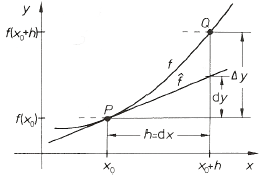
\includegraphics[width=5cm]{images/differential.png}
 
\subsection{Ableitungsregeln}
\renewcommand{\arraystretch}{1.5}
\begin{tabular}{|l|l|}
	\hline \textbf{Konstantenregeln}& $c'=0'$\\
	\hline \textbf{Faktorenregeln}& $(cu)'=c u'$\\
	\hline \textbf{Summenregel}& $(u\pm v)'= u' \pm v'$\\
	\hline \textbf{Produktregel}& $(uv)'=u'v + uv'$\\
	\hline \textbf{Quotientenregel}& $(\frac{u}{v})'= \frac{u'v-uv'}{u^{2}}$\\
	\hline \textbf{Kettenregel}& $y=u(v(x)) ; y'=\frac{du}{dv} \frac{dv}{dx}$\\
	\hline \textbf{Potenzregel} & $(u^{a})'=au^{a-1}$\\
								& $(\frac{1}{u})'= \frac{u'}{u^2}$\\
	\hline	\textbf{Wurzelregel} & $f(x)=\sqrt{x} ; f'(x)=\frac{1}{2\sqrt{x}}$\\
	\hline	\textbf{Logarithmusregel} & $\ln{u}'=\frac{u'}{u}$\\ 
	\hline	\textbf{Differentation der Umkehrfunktion} & $(f^{-1})'(y)=\frac{1}{f'(x)} $\\
	\hline 
\end{tabular}
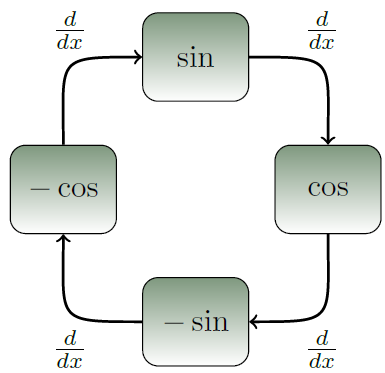
\includegraphics[width=5cm]{images/sin_cos.png}
\newpage
\subsection{Ableitungen elementarer Funktionen}
\renewcommand{\arraystretch}{2.2}
\begin{tabular}{|l|l||l|l|}
	\hline
	\textbf{Funktion} & \textbf{Ableitung} & \textbf{Funktion} &
	\textbf{Ableitung}\\\hline
	\hline $C$ (Konstante) & 0 & $\sec x$ & $\dfrac{\sin x}{\cos^2 x}$ \\
	\hline $x$ & 1 & $\sec^{-1} x$ & $\dfrac{-\cos x}{\sin^2 x}$\\
	\hline $x^n$ ($n\in\mathbb{R}$) & $nx^{n-1}$ & $\arcsin x \quad (|x| < 1)$ &
	 $\dfrac{1}{\sqrt{1-x^2}}$\\
	\hline $\dfrac{1}{x}$ & $-\dfrac{1}{x^2}$ & $\arccos x \quad (|x| < 1)$ &
	$-\dfrac{1}{\sqrt{1-x^2}}$\\
	\hline $\dfrac{1}{x^n}$ & $-\dfrac{n}{x^{n+1}}$ & $\arctan x$ & $\dfrac{1}{1+x^2}$\\
	\hline $\sqrt{x}$ & $\dfrac{1}{2\sqrt{x}}$ & $\arccot{x} $ & $-\dfrac{1}{1+x^2}$\\
	\hline $\sqrt[n]{x}\quad (n\in\mathbb{R}, n \neq 0, x > 0)$ &
	$\dfrac{1}{n\sqrt[n]{x^{n-1}}}$ & $\arcsec x$ & $\dfrac{1}{x\sqrt{x^2-1}}$\\
	\hline $\mathrm{e}^x$ & $\mathrm{e}^x$ & $\arcossec x$ & $-\dfrac{1}{x\sqrt{x^2-1}}$\\
	\hline $\mathrm{e}^{bx}\quad (b\in\mathbb{R})$ & $b\mathrm{e}^{bx}$ & $\sinh x$ &
	$\cosh x$\\
	\hline $a^x\quad (a > 0)$ & $a^x\ln a$ & $\cosh x$ & $\sinh x$\\
	\hline $a^{bx}\quad (b\in\mathbb{R}, a > 0)$ & $ba^{bx}\ln a$ & $\tanh x$ &
	$\dfrac{1}{\cosh^2 x}$\\
	\hline $\ln x$ & $\dfrac{1}{x}$ & $\coth x \quad(x \neq 0)$ & $-\dfrac{1}{\sinh^2 x}$\\
	\hline $\log_a{x} \quad (a > 0, a \neq 1, x > 0)$ &
	$\dfrac{1}{x}\log_a{\mathrm{e}}=\dfrac{1}{x\ln a}$ & $\arsinh x$ &
	$\dfrac{1}{\sqrt{1+x^2}}$\\
	\hline $\lg x \quad (x > 0)$ & $\dfrac{1}{x}\lg \mathrm{e}\approx \dfrac{0.4343}{x}$
	& $\arcosh x \quad (x > 1)$ & $\dfrac{1}{\sqrt{x^2-1}}$\\
	\hline $\sin x$ & $\cos x$ & $\artanh x \quad (|x| < 1)$ & $\dfrac{1}{1-x^2}$\\
	\hline $\cos x$ & $-\sin x$ & $\arcoth x \quad (|x| > 1)$ & $-\dfrac{1}{x^2-1}$\\
	\hline $\tan x \quad (x\neq(2k+1)\dfrac{\pi}{2}, k\in\mathbb{Z})$ & $\dfrac{1}{\cos^2
		x}=\sec^2 x$ & $[f(x)]^n \quad (n\in\mathbb{R})$ & $n[f(x)]^{n-1}f'(x)$\\
	\hline $\cot x \quad (x\neq k\pi, k\in\mathbb{Z})$ & $\dfrac{-1}{\sin^2 x}=-cosec^2x$ & $\ln f(x) \quad (f(x)> 0)$ & $\dfrac{f'(x)}{f(x)}$\\
	\hline
\end{tabular}
\newpage